% 65-25(65쪽) — 반지름 16·중심각 $\theta$ 인 부채꼴 종이로 만든 원뿔(밑면의 반지름 $r$). 스캔 삽화가 흐려 TikZ 로 다시 그림.
% 라벨은 원문 것만: 부채꼴의 $16$·$\theta$, 원뿔 밑면의 $r$. 각도·길이 눈금은 적지 않는다($a+b$ 가 그림에서 읽히지 않게).
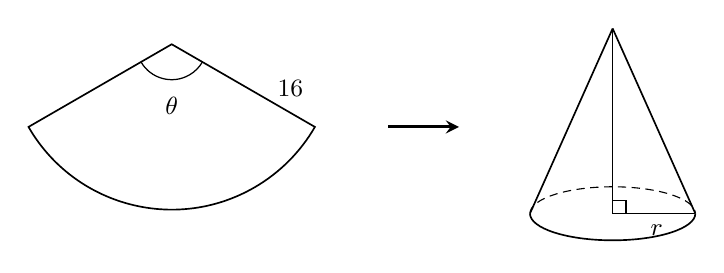
\begin{tikzpicture}[line width=0.6pt, >=stealth]
  % 부채꼴 모양의 종이
  \draw (0,0) -- (-150:2.1) arc (-150:-30:2.1) -- cycle;
  \draw[line width=0.45pt] (-150:0.45) arc (-150:-30:0.45);
  \node[font=\small] at (0,-0.78) {$\theta$};
  \node[anchor=south west, font=\small] at (-33:1.45) {$16$};
  % 접어서 만든다는 표시
  \draw[->, line width=1.1pt] (2.75,-1.05) -- (3.65,-1.05);
  % 원뿔
  \begin{scope}[shift={(5.6,-2.15)}]
    \draw (0,2.35) -- (-1.05,0);
    \draw (0,2.35) -- (1.05,0);
    \draw (-1.05,0) arc (180:360:1.05 and 0.34);
    \draw[densely dashed, line width=0.4pt] (-1.05,0) arc (180:0:1.05 and 0.34);
    \draw[line width=0.5pt] (0,2.35) -- (0,0);
    \draw[line width=0.5pt] (0,0) -- (1.05,0);
    \draw[line width=0.4pt] (0.17,0) -- (0.17,0.17) -- (0,0.17);
    \node[anchor=north, font=\small] at (0.56,-0.02) {$r$};
  \end{scope}
\end{tikzpicture}
